\section{Simulated Samples}
\label{sec:theory}

Monte Carlo (MC) simulations, normalised to the results of the highest order calculations available, are used in the following to compare data to
Z + jets predictions and to estimate the contribution from background events. Signal events, containing a Z boson with associated jets, were simulated using the Sherpa v2.2.1 generator.  Matrix elements were calculated for up to two partons at NLO and up to four additional partons at LO using the Comix and OpenLoops matrix element generators and merged with the Sherpa parton shower using the ME+PS@NLO prescription. The CT10 PDF set was used. Simulated samples of Z+jets production were also produced with the MadGraph5\textunderscore aMC@NLO v2.2.2 generator using explicit matrix elements for up to four partons at leading order, interfaced to the Pythia v8.186 parton shower model. The A14 parton shower tune was used together with the NNPDF23LO PDF set.  The EvtGen v1.2.0 program was used for properties of the bottom and charm hadron decays. The Powheg-Box v2 simulation program, interfaced with the Pythia v8.186 parton shower was also considered. 

The Sherpa v2.2.1 and MadGraph5\textunderscore aMC@NLO v2.2.2 generators are usually favoured over Powheg-Box as they are expected to better model the emission of additional partons. Usage of Sherpa v2.2.1 is strongly advised since the intrinsic parton showering allows for the calculation of up to 2 additional Jets at NLO in addition to the hard process. This formal accuracy is at the cost of additional computing time and as such MadGraph5\textunderscore aMC@NLO is often preferred. 

All generated events are then treated with a full simulation of the ATLAS detector and subsequently physics objects are reconstructed in the same manner as data is. Radiative emissions from muon and taus decays for example are handled by the The PHOTONS++ module within Sherpa. This holds routines to add QED radiation to tau-lepton decays. This has been achieved by an implementation of the YFS algorithm, structured in a way such that the formalism can be extended to scattering processes and to a systematic improvement to higher orders of perturbation theory. The application of PHOTONS++ therefore accounts for corrections that usually are added by the application of PHOTOS to the final state. Figure \ref{fig:ysf}a shows that photon emissions are carefully considered within a MC generator. Figure \ref{fig:ysf}b shows that if detector effects such as isolation and calorimeter calibration are taken into effect. This particular example is covered in detail elsewhere [embedding paper] as the differences between data and simulation need to be well understood especially when comparing the properties of Z$\rightarrow\tau\tau$ and Z$\rightarrow\mu\mu$ decays. 

\begin{figure}[h!]
  \centering
   \subfloat[]{  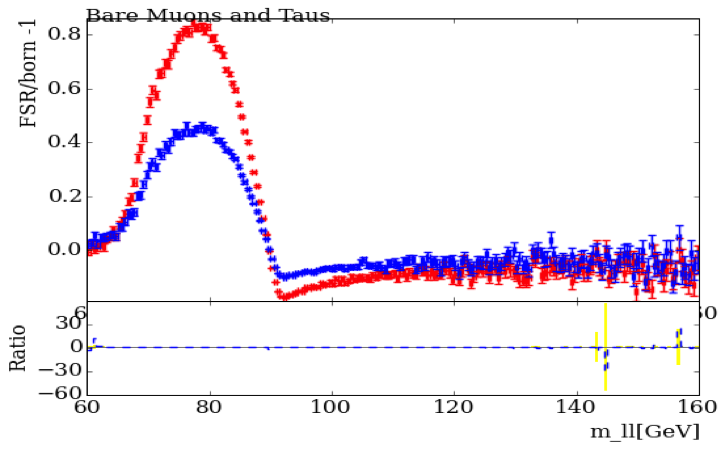
\includegraphics[width=0.49\textwidth]{figures/YFSbare}}
   \subfloat[]{  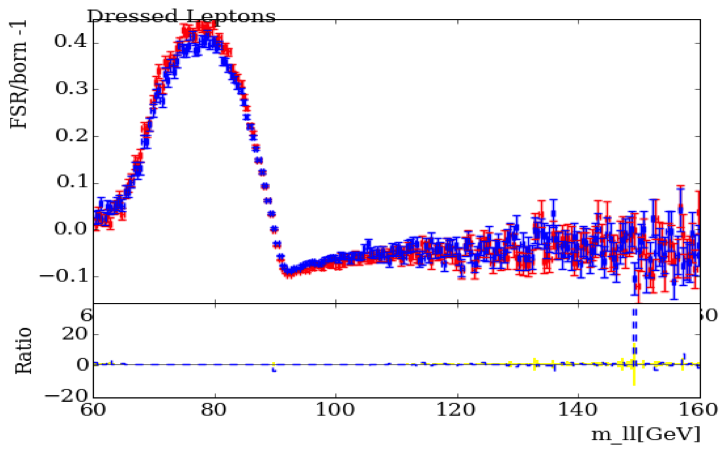
\includegraphics[width=0.49\textwidth]{figures/YFSdressed}}
   \caption{Simulation of Z decays into taus and muons as a ratio of the total cross-section. Plotted is the difference between the masses of the Z boson when radiative corrections are applied. Since the muon is lighter it radiates more energy as seen on the left. When this energy is clustered in a tight calorimeter cone around the lepton; as in the plot on the right, the differences between the two distributions are reconciled}
  \label{fig:ysf}
\end{figure}